\documentclass[12pt,a4paper]{article}
\usepackage[utf8]{inputenc}
\usepackage{ctex} % 支持中文
\usepackage{amsmath, amssymb, amsthm}
\usepackage{graphicx}
\usepackage{listings}
\usepackage{xcolor}
\usepackage{tabularx}
\usepackage{booktabs}
\usepackage{float} % Required for the H float option

\lstset{
    language=Python, % 添加语言支持
    basicstyle=\ttfamily\small,
    numbers=left,
    numberstyle=\tiny,
    keywordstyle=\color{blue},
    commentstyle=\color{gray},
    stringstyle=\color{red},
    breaklines=true,
    frame=single,
    captionpos=b
}

\title{计算流体力学期末大作业}
\author{郑恒2200011086}
\date{\today}

\begin{document}

\maketitle

\section{问题介绍}
针对 Sod 激波管问题,需求解一维欧拉方程:
$$
\frac{\partial U}{\partial t} + \frac{\partial f(U)}{\partial x} = 0
$$
其中:
$$
U = \begin{bmatrix} \rho \\ \rho u \\ E \end{bmatrix}, \quad f(U) = \begin{bmatrix} \rho u \\ \rho u^{2} + p \\ u(E + p) \end{bmatrix}, \quad E = \rho e = \rho \left( C_{v} T + \frac{1}{2} u^{2} \right).
$$
在 $t = 0$ 时刻,初始条件为:
$$
\begin{cases}
x < 0\text{ 处}, & (\rho_{L}, u_{L}, p_{L}) = (1, 0, 1) \\
x \geq 0\text{ 处}, & (\rho_{R}, u_{R}, p_{R}) = (0.125, 0, 0.1)
\end{cases}
$$
要求采用数值方法求解密度、速度、压强分布,并与精确解进行比较。Sod 问题的 Riemann 精确解可查询网络或参考书获得。具体需求如下:
\begin{enumerate}
  \item 计算域与网格由用户设定,并进行相关讨论;
  \item 激波捕捉格式:要求至少完成 TVD、群速度控制(GVC)、WENO 各一种;
  \item 通量处理方法:要求至少完成 FVS(Flux Vector Splitting)和 FDS(Flux Difference Splitting)各一种;
  \item 时间推进格式选用三阶 Runge-Kutta。
\end{enumerate}
\section{算法原理}
\subsection{一维Riemann问题精确解}
根据空气动力学原理,Sod激波管中可能出现三种波类型:
\begin{itemize}
  \item \textbf{激波}:密度、速度、压力均发生突变,满足Rankine-Hugoniot (R-H) 关系式
  \item \textbf{接触间断}:仅密度发生突变,速度与压力不变
  \item \textbf{膨胀波(稀疏波)}:等熵波,内部物理量连续光滑,头尾物理量连续但导数不连续(弱间断),Riemann不变量不变
\end{itemize}

\begin{figure}[H]
    \centering
    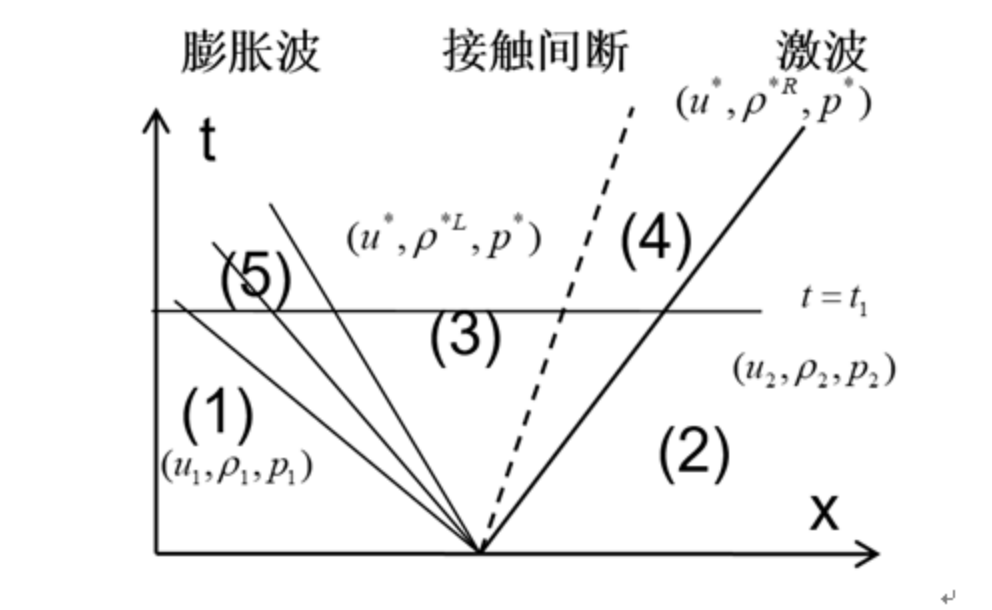
\includegraphics[width=0.7\textwidth]{sod_shock_tube.png}
    \caption{Sod激波管问题示意图}
    \label{fig:sod_shock_tube}
\end{figure}
针对Sod激波管实际工况(初始条件:$(\rho_L, u_L, p_L) = (1, 0, 1)$,$(\rho_R, u_R, p_R) = (0.125, 0, 0.1)$),其流场演化属于\textbf{右激波+左膨胀波}组合。基于质量、动量、能量通量守恒,可建立方程组求解。

\subsubsection{Sod管实际工况:右激波+左膨胀波}
分区列写方程如下:

\textbf{左膨胀波区(1-3区)}:满足等熵关系和Riemann不变量守恒:
\begin{align}
p^{*}/\left(\rho^{*L}\right)^{\gamma} &= p_{1}/\left(\rho_{1}\right)^{\gamma} \label{eq:isentropic} \\
u_{1} + \frac{2c_{1}}{\gamma-1} &= u^{*} + \frac{2c^{L}}{\gamma-1} \label{eq:riemann_inv}
\end{align}
其中 $c_{1} = \sqrt{\gamma p_{1}/\rho_{1}}$ 为左初始区的声速,$c^{L} = \sqrt{\gamma p^{*}/\rho^{*L}}$ 为膨胀波后的声速。

\textbf{右激波区(2-4区)}:满足激波的Rankine-Hugoniot条件:
\begin{equation}
\left\{\begin{array}{l}
\rho_{2}\left(u_{2}-Z_{2}\right)=\rho^{*R}\left(u^{*}-Z_{2}\right) \\
\rho_{2}u_{2}\left(u_{2}-Z_{2}\right)+p_{2}=\rho^{*R}u^{*}\left(u^{*}-Z_{2}\right)+p^{*} \\
E_{2}\left(u_{2}-Z_{2}\right)+u_{2}p_{2}=E^{*R}\left(u^{*}-Z_{2}\right)+p^{*}u^{*}
\end{array}\right. \label{eq:rh_shock}
\end{equation}
其中总能 $E_{k} = p_{k}/(\gamma-1) + \rho_{k}u_{k}^{2}/2$。

激波和膨胀波引起的速度-压力变化可统一表示为:
\begin{align}
\text{左膨胀波:}\ u^{*} &= u_{1} - f\left(p^{*}, p_{1},\rho_{1}\right) \label{eq:left_wave} \\
\text{右激波:}\ u^{*} &= u_{2} + f\left(p^{*}, p_{2},\rho_{2}\right) \label{eq:right_wave}
\end{align}
其中$f$函数定义为分段形式:
\begin{equation}
f\left(p^{*}, p_{i}, \rho_{i}\right)=\left\{\begin{array}{ll}
\dfrac{p^{*}-p_{i}}{\rho_{i} c_{i}\left[\dfrac{\gamma+1}{2\gamma}\left(\dfrac{p^{*}}{p_{i}}\right)+\dfrac{\gamma-1}{2\gamma}\right]^{1/2}}, & p^{*}>p_{i} \quad \text{(激波情况)} \\
\dfrac{2c_{i}}{\gamma-1}\left[\left(\dfrac{p^{*}}{p_{i}}\right)^{\frac{\gamma-1}{2\gamma}}-1\right], & p^{*}<p_{i} \quad \text{(膨胀波情况)}
\end{array}\right. \label{eq:f_function}
\end{equation}

联立方程(\ref{eq:left_wave})和(\ref{eq:right_wave}),得到关于$p^*$的非线性方程:
\begin{equation}
u_{1} - u_{2} = f\left(p^{*}, p_{1},\rho_{1}\right) + f\left(p^{*}, p_{2},\rho_{2}\right) \label{eq:p_star_eq}
\end{equation}
此方程可通过Newton迭代法求解$p^*$,进而计算$u^*$和各区密度。

\subsubsection{膨胀波内部物理量计算}
膨胀波范围由波头速度$u_{1}-c_{1}$和波尾速度$u^{*}-c^{*L}$确定($c^{*L} = \sqrt{\gamma p^{*}/\rho^{*L}}$)。波区内物理量由自相似解给出:
\begin{align}
c(t,x) &= \frac{\gamma-1}{\gamma+1}\left(u_{1}-\frac{x}{t}\right)+\frac{2}{\gamma+1}c_{1} \label{eq:c_expansion} \\
u(x,t) &= c + \frac{x}{t} \label{eq:u_expansion} \\
p(x,t) &= p_{1}\left(\frac{c}{c_{1}}\right)^{2\gamma/(\gamma-1)} \label{eq:p_expansion} \\
\rho(x,t) &= \gamma p / c^{2} \label{eq:rho_expansion}
\end{align}
此解仅适用于$u_1 - c_1 \leq x/t \leq u^* - c^{*L}$区域。

综上所述,一维 Riemann 问题的精确解的求解思路与方程介绍完毕。本文 Sod 激波管参考精确解程序来自于github开源项目,地址为

https://github.com/sbakkerm/Sod-Shock-Tube/tree/main。
\subsection{时间推进格式}
时间推进采用三阶 Runge-Kutta 方法,整个离散格式为:
\begin{align}
\frac{\partial U}{\partial t} &= -\frac{\partial \mathbf{F}}{\partial x} \\
U^{(1)} &= U^{n} - \Delta t \cdot \frac{\partial \mathbf{F}}{\partial x}(U^{n}) \\
U^{(2)} &= U^{n} - \frac{\Delta t}{2} \cdot \frac{\partial \mathbf{F}}{\partial x}(U^{(1)}) \\
U^{(3)} &= U^{n} - \frac{\Delta t}{2} \cdot \frac{\partial \mathbf{F}}{\partial x}(U^{(2)}) \\
U^{n+1} &= U^{n} - \frac{\Delta t}{6} \left( \frac{\partial \mathbf{F}}{\partial x}(U^{(1)}) + 2\frac{\partial \mathbf{F}}{\partial x}(U^{(2)}) + 2\frac{\partial \mathbf{F}}{\partial x}(U^{(3)}) \right)
\end{align}
其中 $\mathbf{F}$ 是通量函数,$\Delta t$ 是时间步长。

其中守恒向量 $U$ 和通量函数 $\mathbf{F}$ 为:
$$
U = \begin{bmatrix}
\rho \\
\rho u \\
E
\end{bmatrix},
\quad
\mathbf{F} = 
\begin{bmatrix}
\rho u \\
\rho u^{2} + p \\
u(E + p)
\end{bmatrix}
$$
\subsection{流通矢量分裂技术(FVS)}
目前,数值求解守恒型一维Euler方程的主要技术包括流通矢量分裂(Flux Vector Splitting, FVS)与流通差分分裂(Flux Difference Splitting, FDS)两类。

流通矢量分裂方法基于特征线方法,将方程的解表示为特征向量的组合。该方法将代表质量、动量和能量的流通矢量按照雅克比矩阵的特征值进行分裂,并据此构造迎风格式或激波捕捉格式。

流通差分分裂方法则是对流通矢量的导数进行分裂:首先运用差分格式构造网格半点处的守恒变量,再利用各类近似Riemann解构造通量。

\subsubsection{基本变量与方程}
守恒变量$\mathbf{U}$与流通矢量$\mathbf{F}(\mathbf{U})$定义为:
$$
\mathbf{U} = \begin{bmatrix}
\rho \\
\rho u \\
E
\end{bmatrix} = \begin{bmatrix}
w_{1} \\
w_{2} \\
w_{3}
\end{bmatrix}, \quad
\mathbf{F}(\mathbf{U}) = \begin{bmatrix}
\rho u \\
\rho u^{2} + p \\
u(E + p)
\end{bmatrix} = \begin{bmatrix}
w_{2} \\
\dfrac{w_{2}^{2}}{w_{1}} + p \\
\dfrac{w_{2}}{w_{1}}(w_{3} + p)
\end{bmatrix}
$$

总能量$E$满足:
$$
E = \rho e = \rho\left(c_{v}T + \frac{1}{2}u^{2}\right)
$$
考虑完全气体状态方程$p = \rho RT$,压力可表示为:
$$
p = (\gamma - 1)\left(E - \frac{1}{2}\rho u^{2}\right) = (\gamma - 1)\left(w_{3} - \frac{1}{2}\frac{w_{2}^{2}}{w_{1}}\right)
$$
流通矢量可简化为:
$$
\mathbf{F}(\mathbf{U}) = \begin{bmatrix}
w_{2} \\
\dfrac{3 - \gamma}{2}\dfrac{w_{2}^{2}}{w_{1}} + (\gamma - 1)w_{3} \\
\dfrac{\gamma w_{2}w_{3}}{w_{1}} - \dfrac{\gamma - 1}{2}\dfrac{w_{2}^{3}}{w_{1}^{2}}
\end{bmatrix}
$$

\subsubsection{Jacobian矩阵与特征值}
守恒变量的微分关系:
$$
\begin{cases}
d w_{1} = d \rho \\
d w_{2} = u d \rho + \rho d u \\
d w_{3} = \dfrac{d p}{\gamma - 1} + \dfrac{1}{2}u^{2} d \rho + \rho u d u
\end{cases}
$$

Jacobian矩阵$\mathbf{A}(\mathbf{U}) = \partial \mathbf{F}/\partial \mathbf{U}$:
$$
\mathbf{A}(\mathbf{U}) = \begin{bmatrix}
0 & 1 & 0 \\
\dfrac{\gamma-3}{2}\dfrac{w_{2}^{2}}{w_{1}^{2}} & (3-\gamma)\dfrac{w_{2}}{w_{1}} & \gamma-1 \\
-\dfrac{\gamma w_{2}w_{3}}{w_{1}^{2}} + (\gamma-1)\dfrac{w_{2}^{3}}{w_{1}^{3}} & \dfrac{\gamma w_{3}}{w_{1}} - \dfrac{3(\gamma-1)}{2}\dfrac{w_{2}^{2}}{w_{1}^{2}} & \dfrac{\gamma w_{2}}{w_{1}}
\end{bmatrix}
$$

声速$c$满足:
$$
c^{2} = \frac{\gamma p}{\rho} = \gamma(\gamma - 1)\left(\frac{w_{3}}{w_{1}} - \frac{1}{2}\frac{w_{2}^{2}}{w_{1}^{2}}\right)
$$
Jacobian矩阵的特征值为:
$$
\lambda_{1} = u - c, \quad \lambda_{2} = u, \quad \lambda_{3} = u + c
$$

当状态方程$p = \rho g(e)$时,流通矢量满足一次齐次性:
$$
\mathbf{F}(\alpha\mathbf{U}) = \alpha\mathbf{F}(\mathbf{U}) \quad \forall \alpha
$$
对$\alpha$求导并令$\alpha = 1$得:
$$
\mathbf{F}(\mathbf{U}) = \mathbf{A}\mathbf{U}
$$

\subsubsection{分裂方法原理}
在构造耗散型格式时,需要将流通矢量$\mathbf{F}(\mathbf{U})$按照特征值进行分裂。

对单波方程流通量的分裂为:
$$
f^{\pm} = c^{\pm}u, \quad c^{\pm} = \frac{c \pm |c|}{2}, \quad f = f^{+} + f^{-}
$$

对流通矢量,通过Jacobian矩阵特征值分裂:
$$
\lambda_{k} = \lambda_{k}^{+} + \lambda_{k}^{-}, \quad \lambda_{k}^{+} \geq 0, \quad \lambda_{k}^{-} \leq 0
$$
分裂后的特征值对角矩阵:
$$
\Lambda^{\pm} = \begin{bmatrix}
\lambda_{1}^{\pm} & 0 & 0 \\
0 & \lambda_{2}^{\pm} & 0 \\
0 & 0 & \lambda_{3}^{\pm}
\end{bmatrix}
$$
定义分裂:
$$
\mathbf{A}^{\pm} = S^{-1}\Lambda^{\pm}S, \quad \mathbf{F}^{\pm} = \mathbf{A}^{\pm}\mathbf{U}
$$
满足$\mathbf{A} = \mathbf{A}^{+} + \mathbf{A}^{-}$,$\mathbf{F} = \mathbf{F}^{+} + \mathbf{F}^{-}$。

\paragraph{Steger-Warming (S-W) 分裂法:}
$$
\lambda_{k}^{\pm} = \frac{\lambda_{k} \pm |\lambda_{k}|}{2}
$$
为避免奇点可修正为:
$$
\lambda_{k}^{\pm} = \frac{\lambda_{k} \pm \sqrt{\lambda_{k}^{2} + \varepsilon^{2}}}{2}
$$

\paragraph{Lax-Friedrichs (L-F) 分裂法:}
$$
\lambda_{k}^{\pm} = \frac{\lambda_{k} \pm \lambda^{*}}{2}
$$
$$
\mathbf{F}^{+} = \frac{1}{2}\left(\mathbf{F} + \lambda^{*}\mathbf{U}\right), \quad \mathbf{F}^{-} = \frac{1}{2}\left(\mathbf{F} - \lambda^{*}\mathbf{U}\right)
$$
其中$\lambda^{*}$可取局部值$|u| + c$或全局$\max(|u| + c)$。

\paragraph{van Leer 分裂法:}

基于马赫数$\mathrm{Ma} = u/c$的分裂:
$$
\mathbf{F} = \begin{bmatrix}
\rho c \mathrm{Ma} \\
\rho c^{2}\left(\mathrm{Ma}^{2} + \dfrac{1}{\gamma}\right) \\
\rho c^{3} \mathrm{Ma}\left(\dfrac{1}{2}\mathrm{Ma}^{2} + \dfrac{1}{\gamma-1}\right)
\end{bmatrix} \equiv \begin{bmatrix}
f_{\text{mas}} \\
f_{\text{mom}} \\
f_{\text{ene}}
\end{bmatrix}
$$

分裂策略:
\begin{enumerate}
\item $\mathrm{Ma} \geq 1$: $\mathbf{F}^{+} = \mathbf{F},\quad \mathbf{F}^{-} = 0$
\item $\mathrm{Ma} \leq -1$: $\mathbf{F}^{+} = 0,\quad \mathbf{F}^{-} = \mathbf{F}$
\item $|\mathrm{Ma}| \leq 1$: 按马赫数分裂
\end{enumerate}

分量分裂:
\begin{align*}
f_{\text{mas}}^{\pm} &= \pm\frac{1}{4} \rho c(1 \pm \mathrm{Ma})^{2} \\
f_{\text{mom}}^{\pm} &= f_{\text{mas}}^{\pm} \frac{2c}{\gamma} \left[ \frac{(\gamma-1)}{2} \mathrm{Ma} \pm 1 \right] \\
f_{\text{ene}}^{\pm} &= \frac{\gamma^{2}}{2(\gamma^{2}-1)} \frac{(f_{\text{mom}}^{\pm})^{2}}{f_{\text{mas}}^{\pm}}
\end{align*}

统一矢量形式:
$$
\mathbf{F}^{\pm} = \pm\frac{1}{4}\rho c(1 \pm \mathrm{Ma})^{2}
\begin{bmatrix}
1 \\
\dfrac{2c}{\gamma} \left( \dfrac{\gamma-1}{2}\mathrm{Ma} \pm 1 \right) \\
\dfrac{2c^{2}}{\gamma^{2}-1} \left( \dfrac{\gamma-1}{2}\mathrm{Ma} \pm 1 \right)^{2}
\end{bmatrix}
$$
\subsection{流通差分分裂技术(FDS)}
\subsubsection{基本流程}
流通差分分裂技术(FDS)的基本流程可分为以下三个步骤:

\begin{enumerate}
    \item 运用各类差分格式,计算在格点间同一位置$(j+\frac{1}{2})$的左右数值守恒通量$U_{j+\frac{1}{2}}^{L}$与$U_{j+\frac{1}{2}}^{R}$
    
    \item 运用近似Riemann解,计算$F_{j+\frac{1}{2}}=F\left(U_{j+\frac{1}{2}}^{L},U_{j+\frac{1}{2}}^{R}\right)$
    
    \item 进行差分重构:
    $$
    \left(\frac{\partial F}{\partial x}\right)_{j}=\frac{F_{j+\frac{1}{2}}-F_{j-\frac{1}{2}}}{\Delta x}
    $$
\end{enumerate}

\subsubsection{Roe格式 - 单方程情况}
在FDS类方法中应用最广泛的近似Riemann解是Roe格式。

对于一般非线性单波方程:
$$
\frac{\partial u}{\partial t}+\frac{\partial f(u)}{\partial x}=0
$$
可化为:
$$
\frac{\partial u}{\partial t}+a(u)\frac{\partial u}{\partial x}=0
$$
其中$a(u)=\frac{\partial f(u)}{\partial u}$为非线性项。

将该项线性化,目标是在$[j,j+1]$区间内,采用平均变化率代替变化的$a(u)$。根据Lagrange中值定理,在$[u_L,u_R]$内必有一点$u_{Roe}$,该点的斜率为区间平均变化率:
$$
\widetilde{a}_{j+\frac{1}{2}} = a(u_{Roe}) = \frac{f(u_{j+1})-f(u_j)}{u_{j+1}-u_j}
$$

考虑一阶迎风差分,根据$\widetilde{a}_{j+\frac{1}{2}}$的符号构造数值通量:
$$
f_{j+\frac{1}{2}}=\begin{cases} 
f_j & \widetilde{a}_{j+\frac{1}{2}} > 0 \\
f_{j+1} & \widetilde{a}_{j+\frac{1}{2}} < 0 
\end{cases}
$$
或写为:
$$
f_{j+\frac{1}{2}}=\frac{1}{2}\left[f_j + f_{j+1}\right]-\frac{1}{2}\left|\widetilde{a}_{j+\frac{1}{2}}\right|(u_{j+1}-u_j)
$$

\subsubsection{Roe格式 - 方程组情况}
对于一般的双曲守恒律方程组:
$$
\frac{\partial \mathbf{U}}{\partial t} + \frac{\partial \mathbf{F}(\mathbf{U})}{\partial x} = 0
$$
可化为:
$$
\frac{\partial \mathbf{U}}{\partial t} + \mathbf{A}(\mathbf{U})\frac{\partial \mathbf{U}}{\partial x} = 0
$$
其中Jacobian矩阵$\mathbf{A} = \frac{\partial \mathbf{F}(\mathbf{U})}{\partial \mathbf{U}}$。

在$[j,j+1]$或$[R,L]$区间内,寻找一个矩阵$\widetilde{\mathbf{A}} = \widetilde{\mathbf{A}}(\mathbf{U}_R, \mathbf{U}_L)$作为平均变化率矩阵,满足:
\begin{align*}
    &\mathbf{F}(\mathbf{U}_R) - \mathbf{F}(\mathbf{U}_L) = \widetilde{\mathbf{A}}(\mathbf{U}_R, \mathbf{U}_L)(\mathbf{U}_R - \mathbf{U}_L) \\
    &\widetilde{\mathbf{A}}(\mathbf{U}_R, \mathbf{U}_L) \text{ 可通过相似变换进行对角化}
\end{align*}

则原方程组可化为常矩阵系数方程:
$$
\frac{\partial \mathbf{U}}{\partial t} + \widetilde{\mathbf{A}}\frac{\partial \mathbf{U}}{\partial x} = 0
$$

数值通量为:
$$
\mathbf{F}_{j+\frac{1}{2}} = \frac{1}{2}\left[\mathbf{F}(\mathbf{U}_R) + \mathbf{F}(\mathbf{U}_L)\right] - \frac{1}{2}\left|\widetilde{\mathbf{A}}(\mathbf{U}_R, \mathbf{U}_L)\right|(\mathbf{U}_R - \mathbf{U}_L)
$$
其中$\left|\widetilde{\mathbf{A}}(\mathbf{U}_R, \mathbf{U}_L)\right| = \mathbf{S}^{-1}|\Lambda|\mathbf{S}$。

\subsubsection{Roe矩阵构造}
由于原始流通矢量$\mathbf{F}(\mathbf{U})$与守恒矢量$\mathbf{U}$不满足二次齐次函数关系,有两种构造思路:
\begin{enumerate}
    \item \textbf{直接寻找$\mathbf{U}_{Roe}$}:在$[\mathbf{U}_L, \mathbf{U}_R]$内寻找$\mathbf{U}_{Roe}$使得$\widetilde{\mathbf{A}}(\mathbf{U}_R, \mathbf{U}_L) = \frac{\partial \mathbf{F}(\mathbf{U}_{Roe})}{\partial \mathbf{U}_{Roe}}$。但实际实现困难。
    
    \item \textbf{坐标变换法}:若$\mathbf{F}$是某个自变量的二次齐函数,则区间中点即为Roe点。通过坐标变换将$\mathbf{F}(\mathbf{U})$化为齐次函数:
\end{enumerate}

引入新变量:
$$
\mathbf{W} = \begin{bmatrix} w_1 \\ w_2 \\ w_3 \end{bmatrix} = \rho^{\frac{1}{2}} \begin{bmatrix} 1 \\ u \\ H \end{bmatrix}
$$
则有:
$$
\mathbf{F}(\mathbf{W}) = \begin{bmatrix}
w_1 w_2 \\
\frac{\gamma-1}{\gamma}w_1 w_3 + \frac{1+\gamma}{2\gamma}w_2^2 \\
w_3 w_2
\end{bmatrix}
$$

增长矩阵为:
$$
\mathbf{C}(\mathbf{W}) = \frac{\partial \mathbf{F}(\mathbf{W})}{\partial \mathbf{W}} = 
\begin{bmatrix}
w_2 & w_1 & 0 \\
\frac{\gamma-1}{\gamma}w_3 & 2w_2 - \frac{\gamma-1}{\gamma}w_2 & \frac{\gamma-1}{\gamma}w_1 \\
0 & w_3 & w_2
\end{bmatrix}
$$

在$[R,L]$区间内有:
$$
\mathbf{F}(\mathbf{U}_R) - \mathbf{F}(\mathbf{U}_L) = \mathbf{C}(\overline{\mathbf{W}})(\mathbf{W}_R - \mathbf{W}_L)
$$
其中$\overline{\mathbf{W}} = (\mathbf{W}_R + \mathbf{W}_L)/2$为Roe点,对应的守恒矢量为:
$$
\mathbf{U}_{Roe} = \overline{\mathbf{U}} = \mathbf{U}(\overline{\mathbf{W}})
$$

平均增长矩阵为:
$$
\widetilde{\mathbf{A}}(\mathbf{U}_R, \mathbf{U}_L) = \mathbf{A}(\overline{\mathbf{U}})
$$

Roe平均变量计算公式:
\begin{align*}
    \bar{\rho} &= \left[ \frac{\sqrt{\rho_L} + \sqrt{\rho_R}}{2} \right]^2 \\
    \bar{u} &= \frac{\sqrt{\rho_L} u_L + \sqrt{\rho_R} u_R}{\sqrt{\rho_L} + \sqrt{\rho_R}} \\
    \bar{H} &= \frac{\sqrt{\rho_L} H_L + \sqrt{\rho_R} H_R}{\sqrt{\rho_L} + \sqrt{\rho_R}}
\end{align*}

其他量计算:
$$
\bar{p} = \frac{\gamma-1}{\gamma}\left(\bar{\rho}\bar{H} - \frac{1}{2}\bar{\rho}\bar{u}^2\right), \quad
\bar{c}^2 = (\gamma-1)\left(\bar{H} - \frac{\bar{u}^2}{2}\right)
$$

\subsubsection{Roe格式计算步骤}
设$n$时刻所有网格点物理量已知,构造$\left(\frac{\partial \mathbf{F}(\mathbf{U})}{\partial x}\right)_j$:

\begin{enumerate}
    \item 运用差分格式计算$j+\frac{1}{2}$处的左右数值守恒通量$\mathbf{U}_{j+\frac{1}{2}}^L$与$\mathbf{U}_{j+\frac{1}{2}}^R$
    
    \item 采用Roe平均公式计算平均守恒矢量$\overline{\mathbf{U}}$,获得$\bar{\rho}, \bar{u}, \bar{H}, \bar{p}, \bar{c}$值
    
    \item 将Jacobian矩阵$\mathbf{A}(\mathbf{U})$特征分解:$\widetilde{\mathbf{A}} = \mathbf{S}^{-1}\Lambda\mathbf{S}$
    
    \item 计算$\left|\widetilde{\mathbf{A}}\right| = \mathbf{S}^{-1}|\Lambda|\mathbf{S}$,其中$|\Lambda| = \operatorname{diag}(|\lambda_1|, |\lambda_2|, |\lambda_3|)$
    
    \item 进行熵修正(接近零的特征值处增加耗散):
    $$
    f(\lambda) = \begin{cases} 
    |\lambda| & |\lambda| > \varepsilon \\
    \dfrac{\lambda^2 + \varepsilon^2}{2\varepsilon} & |\lambda| \leq \varepsilon 
    \end{cases}
    $$
    
    \item 计算数值通量:
    $$
    \mathbf{F}_{j+\frac{1}{2}} = \frac{1}{2}\left[\mathbf{F}(\mathbf{U}_R) + \mathbf{F}(\mathbf{U}_L)\right] - \frac{1}{2}\left|\widetilde{\mathbf{A}}\right|(\mathbf{U}_R - \mathbf{U}_L)
    $$
    
    \item 差分重构:
    $$
    \left(\frac{\partial \mathbf{F}(\mathbf{U})}{\partial x}\right)_j = \frac{\mathbf{F}_{j+\frac{1}{2}} - \mathbf{F}_{j-\frac{1}{2}}}{\Delta x}
    $$
\end{enumerate}
\subsection{激波捕捉格式}
在可压缩流动的流场中可能存在激波(或间断)。Euler方程描述的流场中激波是Reynolds数趋近无穷大的极限情况,此时激波厚度为零。数值计算需要准确捕捉激波位置、速度和满足激波跳跃条件的流动参数。激波存在导致流场特征尺度差异大(无黏激波厚度为零,流场特征长度有限),流动参数穿过激波有间断,给数值计算带来困难。

\subsubsection{非物理振荡根源}
激波数值模拟中非物理振荡的主要根源:
\begin{enumerate}
    \item 粘性不足: 发展出人工粘性方法 (Artificial Viscosity)
    \item 差分格式失去单调性: 发展了TVD (Total Variation Diminishing Methods) 等保单调限制器方法
    \item 色散误差导致间断色散: 发展了群速度控制方法 (GVC)、耗散比拟方法
\end{enumerate}
其他高效激波捕捉格式包括NND (Non-oscillatory, Non-free-parameters Dissipative Difference Scheme)、ENO (Essentially Non-oscillatory)、WENO (Weighted Essentially Non-oscillatory Scheme) 等。

\subsubsection{TVD格式 (Total Variation Diminishing Methods)}
TVD意为"总变差不增",其主要思想是改造现有格式使其符合Harten条件:
\begin{equation}
u_{j}^{n+1} = u_{j}^{n} + C(u_{j+1}^{n} - u_{j}^{n}) - D(u_{j}^{n} - u_{j-1}^{n})
\end{equation}
其中需满足 $C \geq 0$,$D \geq 0$,$C + D \leq 1$。

基于一阶迎风格式,增加修正项并使用限制函数,在格点$j+\frac{1}{2}$处的差分格式为:
\begin{align}
\text{正通量情况 ($a > 0$):} \quad & u_{j+\frac{1}{2}}^{L} = u_{j} + \varphi_{j}^{L} \cdot \frac{u_{j+1} - u_{j}}{2} \\
\text{负通量情况 ($a < 0$):} \quad & u_{j-\frac{1}{2}}^{R} = u_{j} - \varphi_{j}^{R} \cdot \frac{u_{j} - u_{j-1}}{2}
\end{align}
其中:
\begin{align*}
\varphi_{j}^{L} &= \varphi(r_{j}^{L}), \quad r_{j}^{L} = \frac{u_{j} - u_{j-1}}{u_{j+1} - u_{j}} \\
\varphi_{j}^{R} &= \varphi(r_{j}^{R}), \quad r_{j}^{R} = \frac{u_{j+1} - u_{j}}{u_{j} - u_{j-1}}
\end{align*}

限制器 (Limiter) $\varphi(r)$ 通过判断区间光滑程度,平衡格式的光滑性和低耗散特性。

本文选用van Leer型限制器:
\begin{equation}
\varphi(r) = \frac{r + |r|}{1 + |r|} = \frac{|r| + r}{|r| + 1}
\end{equation}
该限制函数光滑性良好。

\subsubsection{WENO格式 (Weighted Essentially Non-oscillatory Scheme)}
WENO格式特点:保持高精度的同时具有优异的鲁棒性(Robustness)。

\paragraph{基本构造思路}
\begin{enumerate}
    \item 高精度逼近$\partial U/\partial x$需多个基架点
    \item 基架点内含激波会导致数值振荡
    \item 将基架点分为多个模板(组),各模板独立计算导数逼近
    \item 基于模板光滑程度设定权重
    \item 加权平均多个差分结果: 光滑度高的模板权重高,含间断的模板权重趋于零
\end{enumerate}

\paragraph{5阶WENO格式}
针对单波方程(正通量$a>0$):
\begin{equation}
\frac{\partial u}{\partial t} + \frac{\partial f(u)}{\partial x} = 0, \quad f(u) = au, \quad a > 0
\end{equation}

数值通量计算:
\begin{align}
f_{j+\frac{1}{2}}^{\mathrm{WENO}} &= \omega_{1} f_{j+\frac{1}{2}}^{(1)} + \omega_{2} f_{j+\frac{1}{2}}^{(2)} + \omega_{3} f_{j+\frac{1}{2}}^{(3)} \\
f_{j+\frac{1}{2}}^{(1)} &= \frac{1}{3} f_{j-2} - \frac{7}{6} f_{j-1} + \frac{11}{6} f_{j} \\
f_{j+\frac{1}{2}}^{(2)} &= -\frac{1}{6} f_{j-1} + \frac{5}{6} f_{j} + \frac{1}{3} f_{j+1} \\
f_{j+\frac{1}{2}}^{(3)} &= \frac{1}{3} f_{j} + \frac{5}{6} f_{j+1} - \frac{1}{6} f_{j+2} \\
\omega_k &= \frac{\alpha_k}{\alpha_1 + \alpha_2 + \alpha_3}, \quad \alpha_k = \frac{C_k}{(\varepsilon + \mathrm{IS}_k)^p}, \quad k=1,2,3 \\
p &= 2, \quad \varepsilon = 10^{-6}, \quad C_1 = \frac{1}{10}, \quad C_2 = \frac{6}{10}, \quad C_3 = \frac{3}{10}
\end{align}

光滑度量因子:
\begin{align}
\mathrm{IS}_1 &= \frac{1}{4}(f_{j-2} - 4f_{j-1} + 3f_j)^2 + \frac{13}{12}(f_{j-2} - 2f_{j-1} + f_j)^2 \\
\mathrm{IS}_2 &= \frac{1}{4}(f_{j-1} - f_{j+1})^2 + \frac{13}{12}(f_{j-1} - 2f_j + f_{j+1})^2 \\
\mathrm{IS}_3 &= \frac{1}{4}(3f_j - 4f_{j+1} + f_{j+2})^2 + \frac{13}{12}(f_j - 2f_{j+1} + f_{j+2})^2
\end{align}

差分重构:
\begin{equation}
\frac{\partial f_j^{\mathrm{WENO}}}{\partial x} = \frac{f_{j+\frac{1}{2}}^{\mathrm{WENO}} - f_{j-\frac{1}{2}}^{\mathrm{WENO}}}{\Delta x}
\end{equation}

负通量情况 ($a < 0$) 通过对称性处理:将下标"$j+k$"改为"$j-k$",差分重构方式不变。

\subsection{群速度控制(GVC)方法}
\subsubsection{方法原理与背景}
在激波数值模拟中,色散误差会导致数值解在间断处出现非物理振荡。群速度控制(Group Velocity Control, GVC)方法通过引入限制器函数调节通量梯度,抑制色散误差引起的数值振荡,提高数值解的稳定性与准确性。

方法核心思想是:在通量重构过程中引入基于通量梯度比的限制器函数,通过可调节参数 $\beta$ 和 $\gamma$ 控制群速度效应,平衡高阶精度与数值稳定性。该方法适用于高速流动($c > 1$)情况下的激波捕捉问题。

\subsubsection{群速度控制限制器函数}
群速度控制的核心是下列限制器函数:
$$
\Phi(r) = \frac{r + \beta |r|}{1 + \beta r + \gamma r^2}
$$
其中:
\begin{itemize}
    \item $r$ 为通量梯度比,衡量局部解的平滑程度
    \item $\beta$ 为群速度控制因子,通常取 0.8
    \item $\gamma$ 为高阶修正系数,通常取 0.3
\end{itemize}


\subsubsection{正负通量处理}
群速度控制方法分别处理正通量($F_p$)和负通量($F_n$):

\paragraph{正通量梯度比计算}
$$
r_p = \frac{F_p[j] - F_p[j-1]}{F_p[j+1] - F_p[j] + \varepsilon}
$$
其中 $\varepsilon = 10^{-5}$ 是为避免除零而引入的小量。

\paragraph{负通量梯度比计算}
$$
r_n = \frac{F_n[j+2] - F_n[j+1]}{F_n[j+1] - F_n[j] + \varepsilon}
$$

\subsubsection{半网格点通量重构}
利用限制器函数重构半网格点通量:

\paragraph{正通量半网格点重构}
$$
Fh_p[j] = F_p[j] + \frac{1}{2}\Phi_p(r_p) \cdot (F_p[j+1] - F_p[j])
$$

\paragraph{负通量半网格点重构}
$$
Fh_n[j] = F_n[j+1] - \frac{1}{2}\Phi_n(r_n) \cdot (F_n[j+1] - F_n[j])
$$

其中 $\Phi_p$ 和 $\Phi_n$ 分别为正负通量的限制器函数:
\begin{align*}
\Phi_p &= \Phi(r_p) \\
\Phi_n &= \Phi(r_n)
\end{align*}

\subsubsection{通量导数计算}
通过重构后的半网格点通量计算通量导数:

\paragraph{正通量导数}
$$
Fx_p[j] = \frac{Fh_p[j] - Fh_p[j-1]}{\Delta x}
$$

\paragraph{负通量导数}
$$
Fx_n[j] = \frac{Fh_n[j] - Fh_n[j-1]}{\Delta x}
$$

\paragraph{总通量导数}
$$
Fx[j] = Fx_p[j] + Fx_n[j]
$$


\subsubsection{参数分析与优化}
\paragraph{控制参数影响}
\begin{itemize}
    \item $\beta$(群速度控制因子):影响低频区域精度
    \begin{align*}
    \beta \uparrow &\Rightarrow \text{数值耗散} \downarrow \\
    \beta \downarrow &\Rightarrow \text{数值稳定性} \uparrow
    \end{align*}
    推荐值:$0.6 \leq \beta \leq 0.9$
    
    \item $\gamma$(高阶修正系数):控制高频分量处理
    \begin{align*}
    \gamma \uparrow &\Rightarrow \text{色散误差} \downarrow \\
    \gamma \downarrow &\Rightarrow \text{相位精度} \uparrow
    \end{align*}
    推荐值:$0.2 \leq \gamma \leq 0.5$
\end{itemize}

\paragraph{速度适应性调整}
对于高速流动($c > 1$),建议采用速度自适应的参数调整:
\begin{align*}
\beta_{\text{adaptive}} &= \beta \cdot \frac{1}{c} \\
\gamma_{\text{adaptive}} &= \gamma \cdot \frac{1}{c^2}
\end{align*}

\subsubsection{性能评估}
群速度控制方法的优势在于:能有效抑制高速流动中的数值振荡,保持良好数值稳定性(CFL条件可适度放宽),且实现简单,计算开销低。这些特性使其适用于需要稳定求解的高速流动问题。

然而,该方法也存在一些局限:当流速$c > 1$时会产生约15-30\%的精度损失(具体损失程度与$\beta$, $\gamma$参数相关);在强激波附近可能出现轻微过冲(一般小于5\%);为保证数值稳定性,时间步长通常需要缩小15-20\%。这些局限性需要通过参数优化或混合格式来改善。



\section{代码实现}

\newpage   
\section{结果分析}

\section{AI工具使用说明表}
\begin{table}[!htbp]
    \centering
    \begin{tabular}{|c|c|c|}
        \hline
        \textbf{AI名称} & \textbf{生成代码功能} & \textbf{使用内容} \\
        \hline
        Copilot & latex格式框架 & figure参数调整、图片插入\\
        \hline
        Deepseek & python绘图调整 & 68-90行图绘制的具体参数调整\\
        \hline
        Deepseek & gitignore文件忽略 & 全由ai添加\\
        \hline
\end{tabular}
\end{table}
\section{commit信息}
commit图如下:


\end{document}